\section{Problem Definition}

Loosely speaking, the high-level objective in transient-detection is to locate intrinsicly(?)-varying objects in each recently shot image of the sky.
More formally and in the concept of this project, this objective can be defined as finding the mapping
\begin{equation}
  \label{eq:def1}
  (I_t,I_s) \longrightarrow S_t 
\end{equation}
where $I_s$ is the recently captured image, namely the \emph{science image}. $I_t$ is the \emph{template} or \emph{reference} iamge, and $S_t$ is the set of \emph{true transients} to be detected.


However, this problem has traditionally been broken down into two subprolems, namely, \emph{image differencing}\footnote{or interchangeably, \emph{difference imaging}} and \emph{smart-thresholding}; the latter being the process of finding a threshold above which all the pixels in the diff image, $I_d$, will be seen as candidate transient sources:
\begin{equation}
  \label{eq:def2}
  (I_t,I_s) \xrightarrow{diff} I_d \xrightarrow{threshold} S_t 
\end{equation}

\begin{figure}[h]
  \centering
  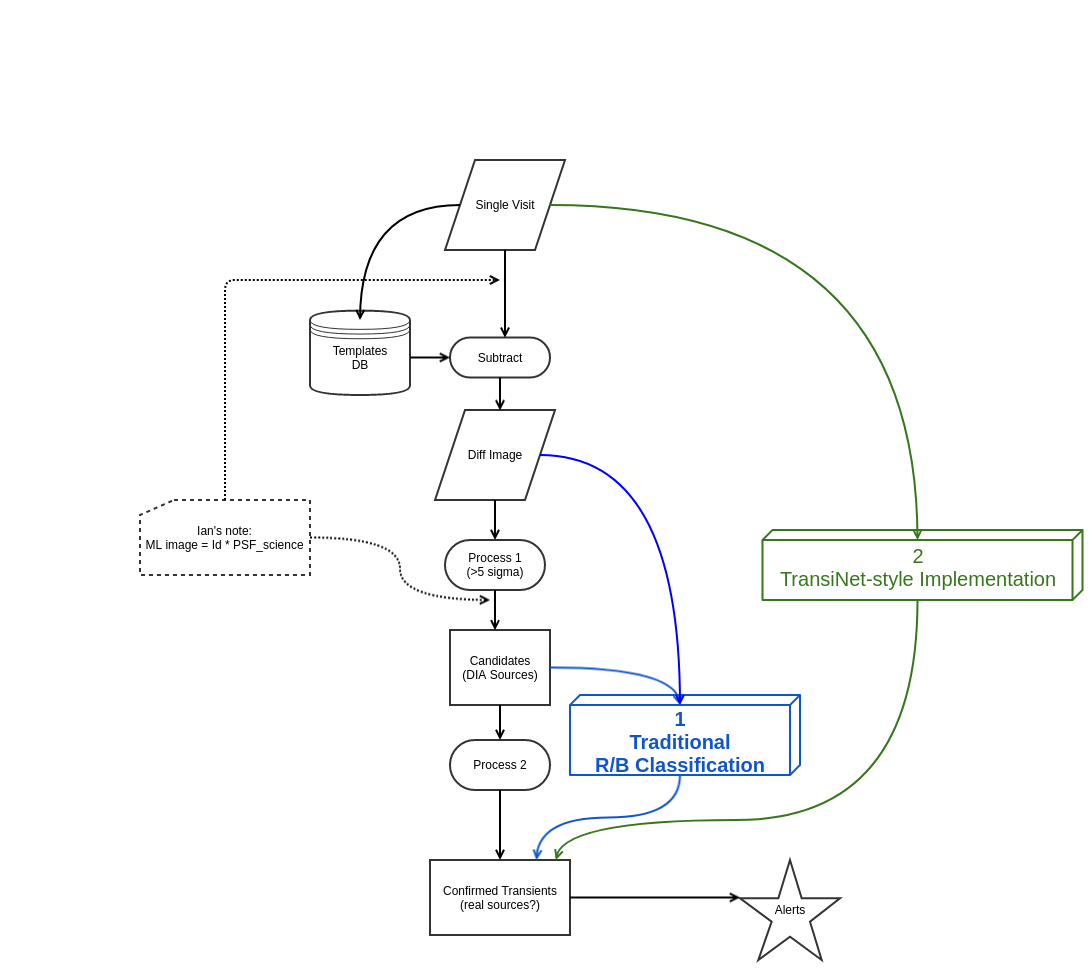
\includegraphics[width=.8\textwidth]{material/diagram}
  \caption{Coarse illustration of information flow through the Alert Production (AP) pipeline. Paths in blue and green illustrate the ``traditional'' and ``modern'' approaches respectively.}
  \label{fig:diagram}
\end{figure}


The \emph{thresholding} step has traditionally been implemented as a simple $5\sigma$-thresholding, but other auxilliary approaches may wrap this stage to make it \emph{smart}er -- figure~\ref{fig:diagram})


\section{Learning-based Approaches}
\label{sec:learning}
The above process is prone to false positives (contamination) and false negatives (misses). Learning-based approaches come into play to mitigate this...

In the context built in the previous section, a learning based approach can be implemented in two broad ways:
\begin{itemize}
\item starting off $I_d$ -- a.k.a traditional real/bogus classification.
\item starting off $(I_t,I_s)$ -- a.k.a end-to-end, TransiNet-style.
\end{itemize}

\footnote{The term 'detection' in the field of computer vision can be translated to localization+classification in the astrophysics' terminology}


each with its own pros and cons..

From a data-scientific perspective, the latter is the preferred and more optimal approach. Pros and cons of the two approaches and details of this preference come in the following sections. However, the current decision is to implement and test the two in parallel. Therefore we shall attempt to bring the two implementations close to eachother -- ideally unified.


\subsection{Basic Real/Bogus Classifier}

\begin{figure}[h]
  \centering
  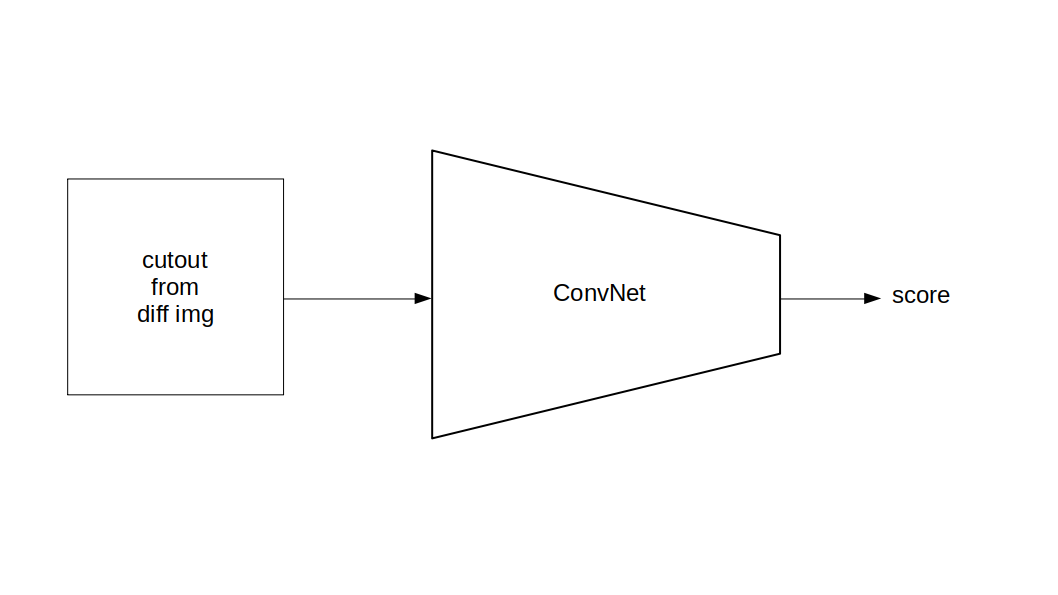
\includegraphics[width=.8\textwidth]{material/rb-classifier}
  \caption{Classical Real/bogus classifier}
  \label{fig:rbdiagram}
\end{figure}

Input-output definition of the problem:
\begin{itemize}
  \item input: cutouts from diff image ($I_d$) with the potential transient at the center
  \item output: reliability score for the potential transient
\end{itemize}

Although the output of a classifier is categorical (i.e. a class label), we will be using the output before the last Softmax~\footnote{TBD} layer, which can be intepretted as a probability.

Features:
\begin{itemize}
  \item can handle single object per cutout -- when there are multiple true transients, the behaviour is ..?
\end{itemize}

\paragraph{The score}
It is foreseeable that the network will eventually learn a concept close to ``PSF-ness'', is it will be processing only spatial data.
% \begin{equation}
%   \[
%     f(x)=
%     \begin{cases}
%       2x^{2018}+9&x<2018\\
%       3x+2018&x\geq 2018.
%     \end{cases}
%   \]
% \end{equation}


\subsection{3D Real/Bogus Classifier}
\begin{figure}[h]
  \centering
  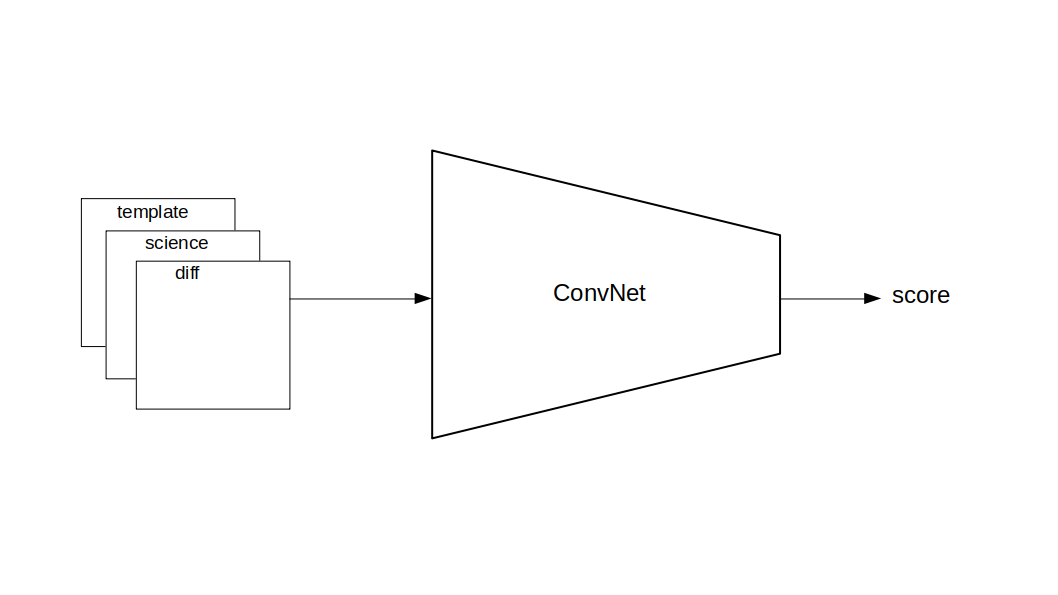
\includegraphics[width=.8\textwidth]{material/rb-classifier-mod}
  \caption{Classical Real/bogus classifier setup can be modified such that corresponding cutouts from template and science images are fed into the network too.}
  \label{fig:rbdiagram}
\end{figure}


\subsection{TransiNet: End-to-End Simultaneous Localization and Classification}

\begin{itemize}
  \item input: single calexp
  \item output: ``score image'': scores are assigned per-pixel
\end{itemize}


\paragraph{The score}
There are bogus detections, variables, ``appearing transients''
\begin{equation}
  s=\left| \frac{A_2-A_1}{A_2+A_1} \right|
\end{equation}




% \section{Notes from the template}

% \subsection{How to handle LSST standard references?} 

% The papers should cite standard LSST references\footnote{See \url{https://github.com/lsst-pst/LSSTreferences}}, 
% where appropriate. For the usage, please see below.  These examples all use the ADS handle, unless they are 
% project docs then the use the project handle like LSE-17.

% All are on the lsst-texmf which you can get from \url{http://lsst-texmf.lsst.io}


% \subsubsection{LSST System and Science}

% The LSST system (brief overview of telescope, camera and data management subsystems),
% science drivers and science forecasts are described in:

% \begin{itemize}
% \item LSST Science Requirements Document: \cite{LPM-17}.
% \item LSST overview paper: \cite{2008arXiv0805.2366I}.
% \item LSST Science Book: \cite{abell2009lsst}.
% \end{itemize}
% %------------------------------------------------------------------------------


% \subsubsection{Simulations}

% The LSST simulations are described in a series of papers. Use of the LSST simulations should cite the LSST simulations overview paper \cite{2014SPIE.9150E..14C} and the specific simulation tools used:

% \begin{itemize}
% \item LSST Catalogs (CatSim): \cite{2014SPIE.9150E..14C}
% \item Feature-Based Scheduler: \cite{2018arXiv181004815N}
% \item Operations Simulator (OpSim): Scheduler \cite{2016SPIE.9910E..13D}, SOCS \cite{2016SPIE.9911E..25R}
% \item Metrics Analysis Framework (MAF): \cite{2014SPIE.9149E..0BJ}
% \item Image simulations (Phosim): \cite{2015ApJS..218...14P}
% \item Sky brightness model: \cite{2016SPIE.9910E..1AY}
% \item LSST Performance for NEO (or moving object) discovery: \cite{2018Icar..303..181J}
% \end{itemize}
% %------------------------------------------------------------------------------


% \subsubsection{Data Management}

% LSST data management system and the data products are described in:

% \begin{itemize}
%   \item The LSST Data Management System: \cite{2015arXiv151207914J}
%   \item Data Products Definition Document: \cite{LSE-163}
% \end{itemize}
%  %------------------------------------------------------------------------------


% \subsubsection{Camera}

% \begin{itemize}
%    \item Design and development of the LSST camera: \cite{2010SPIE.7735E..0JK}
% \end{itemize}
% %------------------------------------------------------------------------------


% \subsubsection{Telescope and Site}

% \begin{itemize}
%    \item Telescope and site overview and status in 2014:  \cite{2014SPIE.9145E..1AG}
% \end{itemize}
% %------------------------------------------------------------------------------

% \subsubsection{System Engineering}

% \begin{itemize}
%    \item LSST systems engineering: \cite{2014SPIE.9150E..0MC}
%    \item System verification and validation: \cite{2014SPIE.9150E..0NS}
% \end{itemize}
% %


